\label{sec:intro}
Consider the stochastic shortest path problem~\citep{bertsekas1991analysis} where an agent learns to cross a frozen lake while avoiding patches of weak ice. The agent can either cross the ice directly, or take the longer, safer route circumnavigating the lake.  The agent is provided with aerial images of the lake, which include color variations at patches of weak ice.  To cross the lake, the agent must learn to identify its own position, goal position, and the location of weak ice from the images.  Even for this simple environment, high-dimensional inputs and sparse rewards can make learning a suitable policy computationally expensive and sample inefficient.  Therefore one might instead efficiently learn, in simulation, an omniscient \emph{expert}, conditioned on a low-dimensional vector which fully describes the state of the world, to complete the task. A \emph{trainee}, observing only images, can then learn to mimic the actions of the expert using sample-efficient online imitation learning~\citep{Ross2011}. This yields a high-performing trainee, conditioned on images, learned with fewer environment interactions overall compared to direct reinforcement learning (RL). 

While appealing, this approach can fail in environments where the expert has access to information unavailable to the agent, referred to as \emph{asymmetric information}.  Consider instead that the image of the lake does not indicate the location of the weak ice.  The trainee now operates under increased uncertainty.  This results in a different optimal partially observing policy, as the agent should now circumnavigate the lake.  However, imitating the expert forces the trainee to always cross the lake, despite being unable to locate and avoid the weak ice. Even though the expert is optimal under full information, the supervision provided to the trainee through imitation learning is poor and yields a policy that is not optimal under partial information. The key insight is that \emph{the expert has no knowledge of what the trainee does not know}.  Therefore, the expert cannot provide suitable supervision, and proposes actions that are not robust to the increased uncertainty under partial information. The main algorithmic contribution we present follows from this insight: the \emph{expert} must be refined based on the behavior of the \emph{trainee} imitating it.

Building on this insight, we present a new algorithm: adaptive asymmetric DAgger (A2D), illustrated in Figure \ref{fig:a2d}.  A2D extends imitation learning by refining the expert policy, such that the resulting supervision moves the trainee policy closer to the optimal \emph{partially observed} policy.  This allows us to safely take advantage of asymmetric information in imitation learning.  Crucially, A2D can be easily integrated with a variety of different RL algorithms, does not require any pretrained artifacts, policies or example trajectories, and does not take computationally expensive and high-variance RL steps in the trainee policy network.  

\begin{figure*}
    \centering
    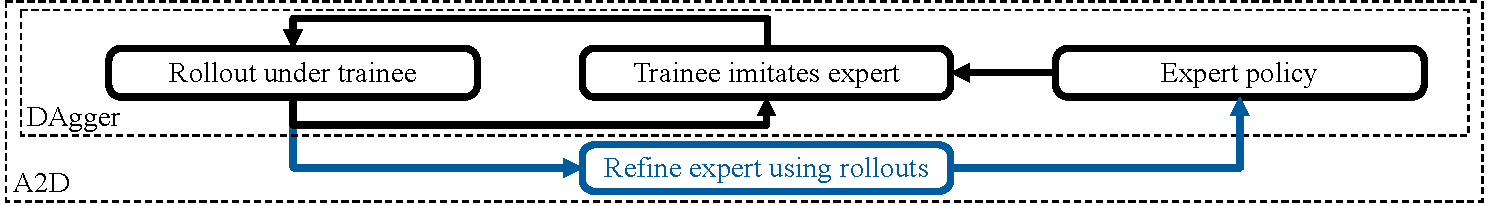
\includegraphics[width=\textwidth]{figures/ad_vs_a2d_super_simple.pdf}
    \vspace*{-0.3cm}
    \caption{Flow chart describing adaptive asymmetric DAgger (A2D), introduced in this work, which builds on DAgger~\citep{Ross2011} by further refining the expert conditioned on the trainee's policy. }
    \label{fig:a2d}
\end{figure*}

We first introduce asymmetric imitation learning (AIL).  AIL uses an expert, conditioned on full state information, to supervise learning a trainee, conditioned on partial information.  We show that the solution to the AIL objective is a posterior inference over the true state; and provide sufficient conditions for when the expert is guaranteed to provide correct supervision.  Using these insights, we then derive the theoretical A2D update to the expert policy parameters in terms of Q functions.  This update maximizes the reward of the trainee implicitly defined through AIL.  We then modify this update to use Monte Carlo rollouts and GAE~\citep{schulman2015high} in place of Q functions, thereby reducing the dependence on function approximators. 

We apply A2D to two pedagogical gridworld environments, and an autonomous vehicle scenario, where AIL fails. We show A2D recovers the optimal partially observed policy with fewer samples, lower computational cost, and less variance compared to similar methods.  These experiments demonstrate the efficacy of A2D, which makes learning via imitation and reinforcement safer and more efficient, even in difficult high dimensional control problems such as autonomous driving. Code and additional materials are available at \url{https://github.com/plai-group/a2d}.
